\chapter{Design and implementation}
\label{chap:design}

\section{System architecture}
\label{sec:sysarch}

\subsection{Top level}

\begin{figure}
  \centering
  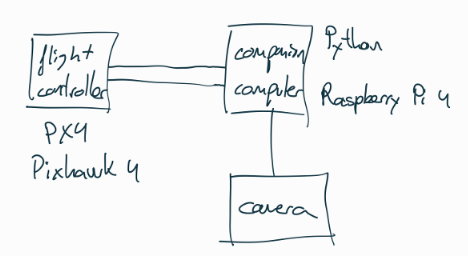
\includegraphics[keepaspectratio]{img/toplevel-sysarch.png}
  \caption{Top level diagram of the hardware/software interactions \todo[inline]{Draft}}\label{fig:toplevel}
\end{figure}

The purpose of the Dronecontrol application is to be able to direct the movement of a \gls{uav} through the analysis of the images taken by a camera.
Since the processing power needed to work with the images recorded is superior to that offered by the autopilot flight controller it becomes necessary the use of an additional companion computer that will control the camera and employ machine learning to extract useful features from the images, as well as transform those features into movement directives for the vehicle.

A top level diagram of the individual parts that comprise the system is shown in Figure~\ref{fig:toplevel}. The main elements are the flight controller, that will run the PX4 autopilot \ref{subsec:px4}, the companion computer, that will run the developed application, and the camera, which provides the images.
The flight controller interfaces directly with the companion computer using the \gls{mavlink} protocol described in Section~\ref{subsec:mavlink}, either through a wireless radio link or a cabled serial connection between the two.
The camera is connected to the companion computer through a cable into an USB port on the computer.
Typically, the type of connection between the flight controller and the computer depends on the desired setup for the system so in the case where the camera, and therefore the companion computer, flies onboard the vehicle it is most convenient to use a direct wire connection between the two, as it provides a faster and more stable link. 
This onboard configuration is further detailed in Section~\ref{subsec:offboard}.
On the other hand, in the case where the companion computer will be acting more like a ground station on an offboard configuration it becomes strictly necessary to communicate with the flight controller through a wireless connection. For this purpose, a pair of telemetry radios provided with the Development Kit of the Holybro X500 (\ref{subsec:pixhawk}) are used. The complete setup requiered for this configuration is described in Section~\ref{subsec:onboard}.

In this project, the flight controller is driven by the PX4 software (\ref{subsec:px4}) and the hardware employed is optimized for this flight stack.
PX4 uses sensors to determine the vehicle state, which is needed for stabilization and to enable autonomous control.
It minimally requires a gyroscope, accelerometer, magnetometer (compass) and barometer.
A GPS or other positioning system is needed to enable all automatic flight modes, and some assisted ones.
PX4 uses outputs to control motor speed, flight surfaces like ailerons and flaps, camera triggers, parachutes, grippers, and many other types of payloads.
Many PX4 drones use brushless motors that are driven by the flight controller via an Electronic Speed Controller (ESC).
The ESC converts a signal from the flight controller to an appropriate level of power delivered to the motor.
PX4 drones are mostly commonly powered from Lithium-Polymer (LiPo) batteries.
The battery is typically connected to the system using a Power Module or Power Management Board, 
which provide separate power for the flight controller and to the ESCs for the motors.
A Radio Control (RC) system is used to manually control the vehicle.
It consists of a remote control unit that uses a transmitter to communicate stick/control positions with a receiver based on the vehicle.
Some RC systems can additionally receive telemetry information back from the autopilot.
Telemetry Radios can provide a wireless MAVLink connection between a ground control station and a vehicle running PX4.
This makes it possible to tune parameters while a vehicle is in flight, inspect telemetry in real-time, change a mission on the fly, etc.

On an actual UAV, the PX4 software runs on a dedicated piece of hardware like the Pixhawk 4 flight controller described in Section~\ref{subsec:pixhawk} that includes all the minimal required sensors for flight as well as interfaces to connect additional actuators and I/O systems (RC, telemetry radio, etc).
However, it is also possible to simulate this hardware on a standard Linux system by building the PX4 source code on a computer with this operating system.
This process is described in the development environment section (\ref{sec:devenv}).

The Dronecontrol application that runs on the companion computer has been developed using the Python programming language \footnote{\url{https://www.python.org/}}.
It offers good advantages for a project of this characteristics because of its high-level,
easy-to-use syntax, that usually results in a smaller code base than other comparable languages for small projects, its versatility and support for object-oriented programming. 
Most importantly, Python is widely used and its official package manager \gls{pip} greatly simplifies the use of external libraries and which gathers in its package index \footnote{\url{https://pypi.org/}} thousands of standard utilities,
including many machine learning and image processing projects and all the required libraries for interacting with PX4 through the MAVLink protocol (MavSDK).
As it is an interpreted language, it can run easily in any system with Python installed without the need to compile separate binaries for different operating systems.

The next sections explore deeper into the differences between the two configurations mentioned before: offboard computer (or ground station) and onboard computer.

\subsection{Offboard configuration}
\label{subsec:offboard}

The offboard configuration allows the flight controller to communicate and receive orders from a companion computer that is not physically connected to its hardware but that can instead stay on ground while the vehicle flies.
This has the advantage that it permits a simpler configuration, without having to be concerned with low-level hardware interactions between the two systems or powering of the companion computer while in flight, as well as allowing the use of a more powerful computer for image processing.
However, it also requires that the camera stays connected to computer on the ground so it cannot use images from the perspective of the drone in flight which limits the real-world applications of the system.
Other configurations involving a direct connection from a camera to the flight controller and the transmission of its images wirelessly to the companion computer through mavlink for processing can be feasible with the current technology but fall out of the scope of this project.

The wireless link is established in this instance through a pair of telemetry radios that connect to a telemetry port on the flight controller and to a USB port in the companion computer, respectively.
Since the Pixhawk 4 is configured by default to used its \verb|TELEM1| port for this purpose, no additional configuration is needed when using that port.
In the companion computer, applications like the QGRoundControl \footnote{\url{http://qgroundcontrol.com/}} ground station software which is part of the Dronecode Project are able to detect automatically a telemetry radio inserted into any of the USB ports of the host computer.
Additionally, other applications using the MavSDK (\ref{subsec:mavlink}) library can establish connection specifying the baudrate and the USB serial port address, usually something similar to \verb|/dev/ttyUSB0| on Linux and \verb|COM#| on Windows.

The radio used for the physical tests in this project is the Holybro SiK Telemetry Radio \footnote{\url{http://www.holybro.com/product/transceiver-telemetry-radio-v3/}}.
It is a small, light and inexpensive open source radio platform that typically allows ranges of better than 300m “out of the box” (the range can be extended to several kilometres with the use of a patch antenna on the ground).
The radios are offered either as 915Mhz (Europe) or 433Mhz (US) so they can be used in different regions and comply with the regulations for frequency, hopping channels and power levels.
They offer 2-way full-duplex communication through an adaptive TDM UART interface and their antenna allows for an adjustable 100-mW-maximum output power and -117 dBm receive sensitivity.
The link is established by default with a baudrate of 57600 (max bits per second on a serial channel) and it can provide air data rates of up to 250 kbps.

\todo[inline]{Images of the radios}
\todo[inline]{Images of the flight controller}
\todo[inline]{Connection diagram / pictures}

\subsection{Onboard configuration}
\label{subsec:onboard}

The second way of configuring the interaction between the flight controller and the companion computer consists of integrating both together on board the \gls{uav}.
In this case, the connection is done through a direct cable between the serial port in the flight controller and a USB port in the companion computer.
The camera will then be connected via cable as well to the companion computer and oriented in the vehicle in a way that allows for the best possible perspective during flight.
This configuration makes it possible to develop new control solutions based on images taken directly from the vehicle and that reflect the trajectory that it follows.
Therefore, it becomes possible to adjust the control loop based on previous reactions of the vehicle to commands and maintain a feedback loop for a more stable guidance.

Since the computer running the visual processing algorithm now has to fly on board the vehicle, it becomes specially important to make a good choice when selecting hardware.
To be able to take into the air, the computer has to be light enough that its weight can be lifted by the propellers while maintaining an adequate battery autonomy, but also powerful enough that the processor can handle the computer vision algorithms required to extract the necessary features from the images taken from the onboard camera that are to be feed to the control loop.

\begin{figure}
  \centering
  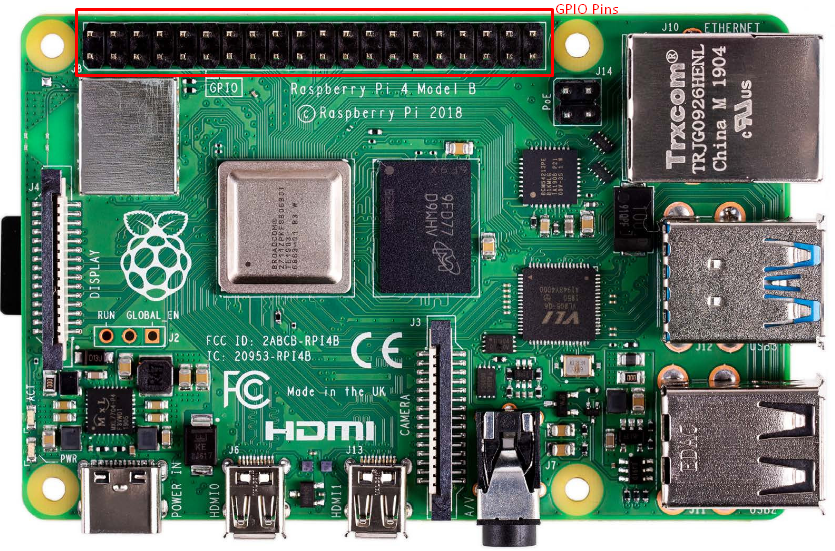
\includegraphics[width=\textwidth,keepaspectratio]{img/rpi4.png}
  \caption{The Raspberry Pi 4 microcomputer, with its 40-pin GPIO header marked in red}\label{fig:rpi4}
\end{figure}
\todo[inline]{Add pinout figure}
The Raspberry Pi 4 model chosen for this project and shown in Figure~\ref{fig:rpi4} is one of the most popular small computers available in the market at the time and it is widely use in all kinds of robotics projects both for education and hobbyists.
One of the most important advantages of using such a platform is the easy access to a great amount of manuals, guides and other support available online.
In addition, the Raspberry's officially supported operating system, called Raspberry Pi OS, is a Debian-based version of Unix optimized for its ARM microcontroller, which simplifies the process of moving from an Ubuntu test environment into real flight experiments.
Since this computer is designed to be easy to integrate with hardware projects it includes a 40-pin GPIO header (marked in red in Figure~\ref{fig:rpi4}) that can be programmed for connecting to any number of external devices.

The Raspberry Pi is powered by a 5V input that can be provided either from its USB-C port or through one of two pins in the header dedicated to this (marked as DC 5v power on Figure~\ref{fig:pinout}.
In the case of the particular vehicle build used in this project, the power management board used (the Holybro PM07 \footnote{\url{http://www.holybro.com/product/pixhawk-4-power-module-pm07/}}) also provides 5V to the flight controller, as well as powering the ESCs to the motors, and counts with two power outputs so one of them can be connected to the flight controller's \verb|POWER1| port and the other to the Raspberry Pi's pins through a custom-made connector.
\todo[inline]{Power management: more about this when it works}

In regards to the camera that will fly onboard the vehicle, there are many possibilities to chose from.
The most important characteristics that should be looked for are a small weight and simple plug-and-play interaction with the onboard computer.
For the tests carried out and detailed in Section~\ref{chap:validation} a Logitech 1080p webcam \todo{Exact model and link} has been used.
Since the frame of the Holybro X500 is not prepared by default to include an onboard camera, it became necessary to design a support to hang from the central rods of the vehicle frame where the camera could be attached securely during flight.
\todo[inline]{Pictures and 3D model}

\begin{figure}
  \centering
  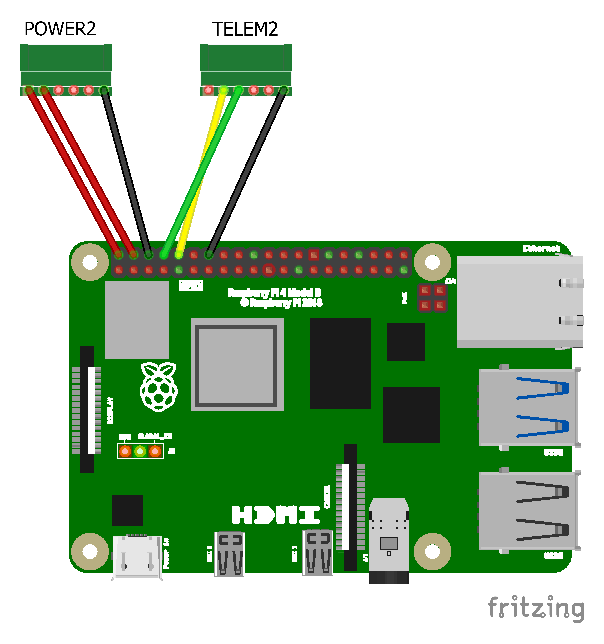
\includegraphics[keepaspectratio]{img/wiring-diagram.pdf}
  \caption{A diagram of the wired connections from the Raspberry Pi 4 to the power management board (TELEM1) and the flight controller (TELEM2).}\label{fig:wiring}
\end{figure}
The second wired connection that needs to be established for this configuration is between the flight controller and the companion computer so the Mavlink messages can be exchanged.
As it is desirable to be able to maintain a wireless link to the vehicle even while it is being controlled by the onboard computer, the telemetry radio is kept connected to the \verb|TELEM1| port of the flight controller and the companion computer is wired to the \verb|TELEM2| port.
This port is not configured to be used by default so it is necessary to modify the configuration of the Pixhawk board either through QGroundControl \todo{More about QGC in SotA} or the PX4 console. \todo{More about this in validation ????}
The other end of the connector has three female Dupont wires that go into the TX/RX UART pins of the Raspberry Pi.
A diagram of the connections to the companion computer can be seen in Figure~\ref{fig:wiring}.
\todo[inline]{Description of 6 wires from connectors both power and telem}

In comparison with the default baudrate of 57600 on the telemetry radio link established in the previous section the wired serial connection works at a baudrate of 921600, which means the data is transferred 16 times faster through the link.
\todo{Main limitation is image processing though, so slower processing power from computer means slower responsiveness to movement all together. Any info about update rate from PX4? Does it depend on the link speed or is it constant?}
\todo[inline]{Link to section in validation where onboard setup is done}

The offboard configuration allowed the supervision of the output from the program while the vehicle was flying, since the computer stayed stationary on the ground, however in this configuration it is not possible to have a screen connected directly to the companion computer.
To fix this situation and be able to monitor during flight, as well as being able to give input directly to the program, it is possible to make use of the WiFi receptor of the Raspberry Pi to configure a remote desktop and connect to it through another computer serving as a ground station;
then the output from the camera and the image recognition can be seen in real time.
A more detailed description of the configuration required can be found on Section~\ref{sec:devenv}.

\section{Development environment and simulation}
\label{sec:devenv}
During the process of developing the application, it became necessary to be able to continuously deploy and test the latest version without having to depend on flying the physical vehicle, but instead relying on the simulation of the system inside the computer that was at the same time running the developed software.
This configuration has the twofold advantage of reducing the development time on the one hand, since there is no need to be concerned with the interactions between the different hardware components and the results can be visualized immediately in the computer screen, and on the other hand of increasing the safety of the process by only running on the vehicle software that has already been tested to an acceptable point.

Simulators allow PX4 flight code to control a computer modeled vehicle in a simulated "world" that can be interacted with in the same ways as with a real vehicle, using QGroundControl, an offboard API, or a radio controller/gamepad. PX4 supports two different simulation modes: software-in-the-loop (\gls{sitl}), where the flight stack runs on a computer, and hardware-in-the-loop (\gls{hitl}), where it uses a simulation firmware on a real flight controller board.
\begin{figure}
  \centering
  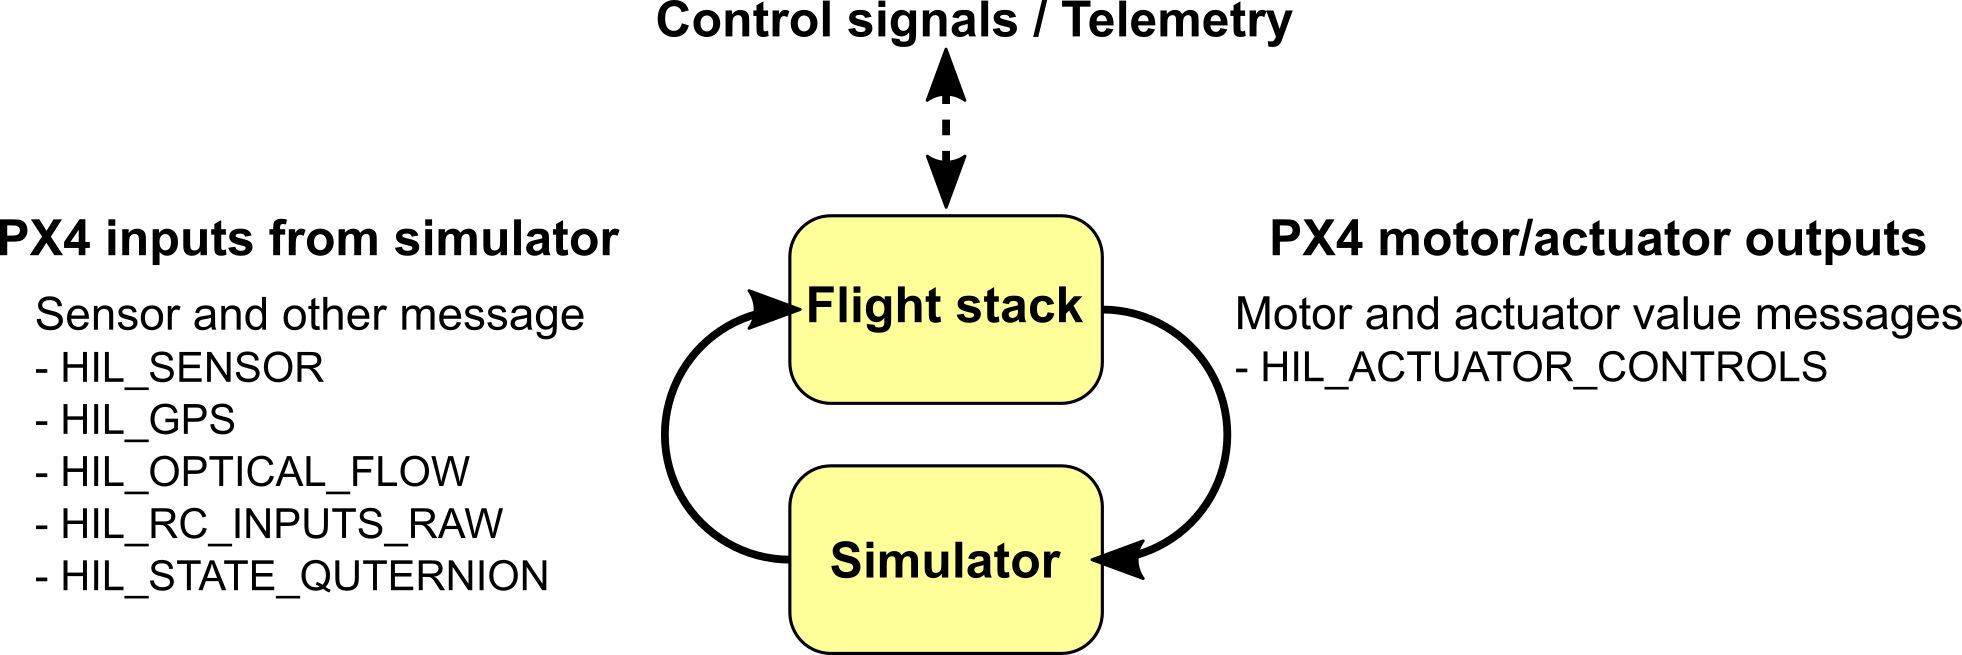
\includegraphics[width=\textwidth,keepaspectratio]{img/px4_simulator_messages.png}
  \caption{Mavlink messages exchanged between the simulator and the flight stack during simulation.}\label{fig:simulator-msgs}
\end{figure}
In both modes, the simulation works according to the feedback loop shown in Figure~\ref{fig:simulator-msgs}. 
The simulator generates the input from the sensors based on its internal world representation and sends it through Mavlink messages to the flight stack running on the same computer using the \gls{udp} transport protocol, which in turn generates response actuator controls that are fed back into the simulator in the same way to affect the vehicles position, velocity and attitude in the simulated world.
\todo[inline]{Explain more about how mavlink protocol works (messages) ???? On SotA ????}

There are many options for simulators supported by PX4 like Gazebo, a powerful 3D simulation environment for Linux systems that is particularly suited for testing object-avoidance and is commonly used with ROS, or AirSim (\ref{subsec:airsim}), a more resource-intensive cross-platform simulator that leverages the Unreal Engine, typically used for game development and animation to provides physically and visually realistic simulations.
For this project AirSim was chosen because of previous experience with Unreal Engine as well as for the easy availability of visual packages to test computer vision features and its native support for running on Windows machines, which is the operating system running on the computer where the tests will take place.
AirSim offers as well a Python library called airlib (\footnote{\url{https://pypi.org/project/airsim/}}) that can be used to retrieve images taken from a simulated camera from the perspective of the drone in the simulation world.
This feature will be necessary when testing the person-recognition utilities used in the program.
\begin{figure}
  \centering
  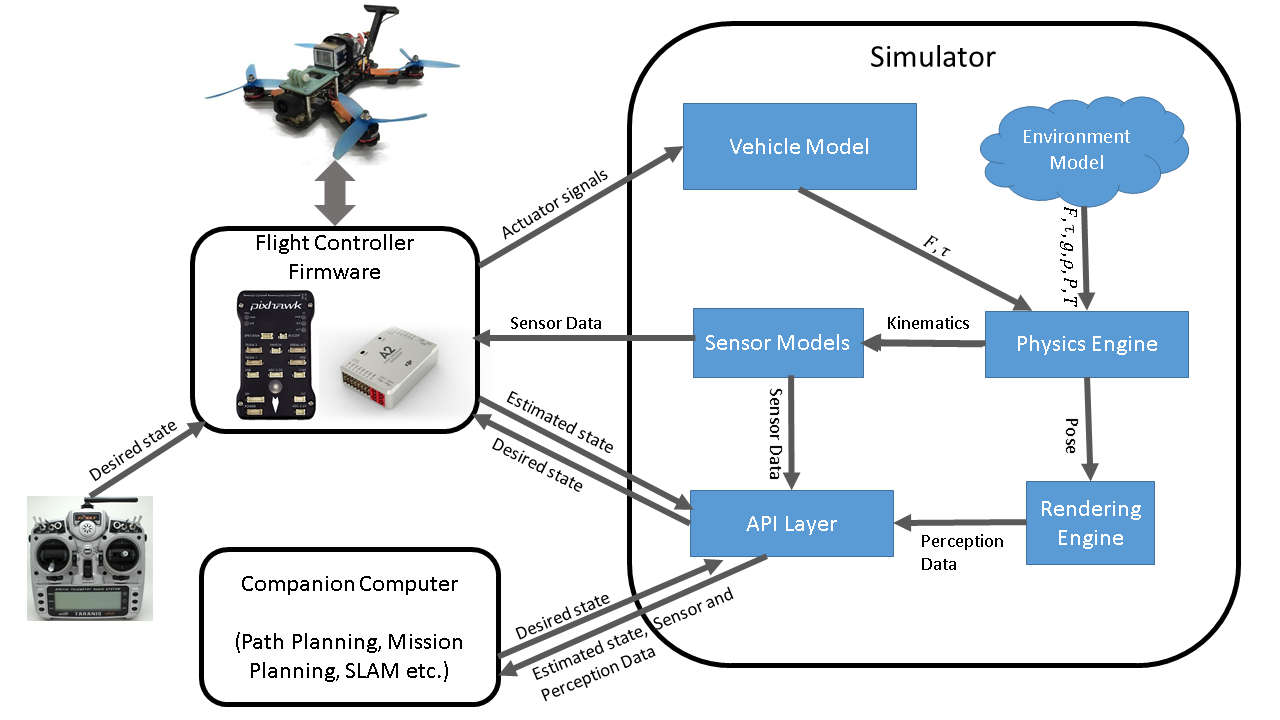
\includegraphics[width=\textwidth,keepaspectratio]{img/airsim-overview.png}
  \caption{High level overview of how different components interact with each other in the AirSim simulator.}\label{fig:airsim-overview}
\end{figure}
A high level overview of the simulator architecture and the way different components interact with each other can be seen in Figure~\ref{fig:airsim-overview}. 
The API layer present in the Figure inside the simulator environment refers to AirSim's own airlib library, which exposes with high-level functionality to send control commands to the flight controller directly.
However, in order to share the same control code when simulating flight and in real flight without and not depend on the simulator system, the control commands are sent using the official MavSDK API instead, which allows communication of estimated state, desired state and sensor data directly between the flight controller firmware and the companion computer.

In order to run software-in-the-loop simulation, the PX4 firmware needs to be built from the source code on the Linux platform where it is going to run.
The build system then sets up all the necessary ports for the Mavlink communication and starts a local instance of the NuttX operating system that runs on the actual flight board.
\begin{figure}
  \centering
  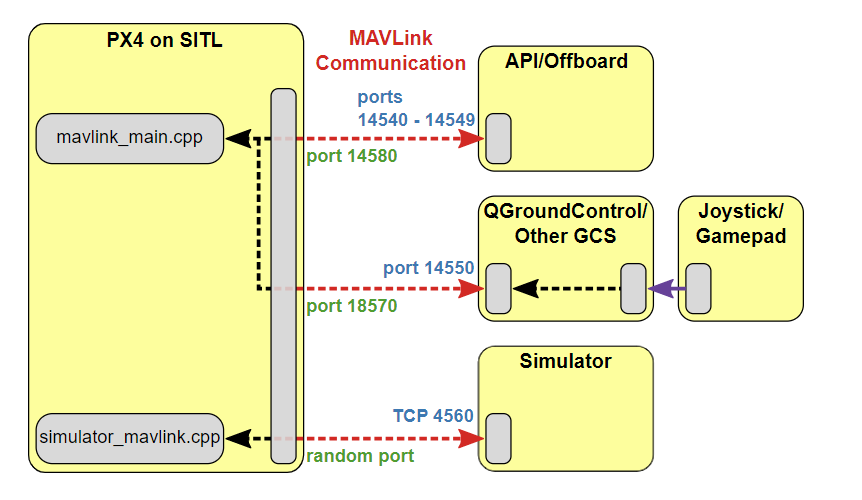
\includegraphics[width=\textwidth,keepaspectratio]{img/px4-ports.png}
  \caption{Network diagram between the different components that interconnect during software-in-the-loop simulation.}\label{fig:px4-ports}
\end{figure}
Figure~\ref{fig:px4-ports} shows how the different parts of the system communicate with each other inside a SITL simulation.
PX4 uses commonly established UDP ports for MAVLink communication with ground control stations (e.g. QGroundControl), offboard APIs (e.g. MAVSDK, MAVROS) and simulator APIs (e.g. AirSim, Gazebo).
External developer application like Dronecontrol use an offboard API, in this case MAVSDK, and therefore listen to PX4's remote UDP port 14540.
All ports in the range 14540-14549 can be used to connect offboard API, for example in the case of controlling multiple vehicles at the same time.
PX4's remote UDP Port 14550 is used for communication with ground control stations, which are expected to listen for connections on this port (QGroundControl listens to this port by default).
PX4 uses a simulation-specific module to connect to the simulator's local TCP port 4560. 
Simulators then exchange information with PX4 using the Simulator MAVLink API shown in Figure~\ref{fig:simulator-msgs}. 
PX4 on SITL and the simulator can run on either the same computer or different computers on the same network.

Since the purpose of using AirSim as a simulator is to run it on a Windows computer and the PX4 software-in-the-loop stack runs on Linux, it is necessary to run a virtualized Linux OS in parallel on the Windows computer and setup a local network so that the simulator and the flight controller firmware can communicate with each other.
The PX4 development team officially supports running the SITL flight stack in Windows through the Windows Subsystem for Linux (WSL2)\footnote{\url{https://docs.microsoft.com/en-us/windows/wsl/about}}, which allows users to install and run their Ubuntu Development Environment on Windows as if it was running it on a Linux computer.
The Windows Subsystem for Linux lets developers run a GNU/Linux environment (including most command-line tools, utilities, and applications) directly on Windows, unmodified, without the overhead of a traditional virtual machine or dualboot setup.
The full steps needed for to configure the system are detailed in Section~\ref{sec:test2}.

\begin{figure}
  \centering
  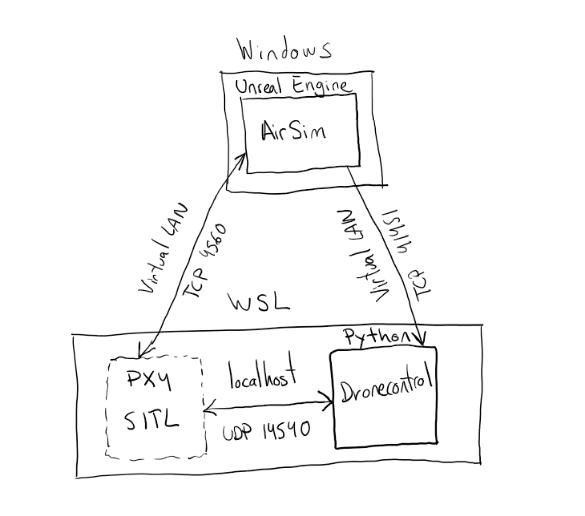
\includegraphics[scale=0.8,keepaspectratio]{img/sitl-connections.png}
  \caption{Connection diagram of how the three systems that interact with each other during SITL simulation.}\label{fig:sitl-connections}
\end{figure}
The whole set of connections established in the software-in-the-loop simulation is shown in Figure~\ref{fig:sitl-connections} at the transport layer level. The two systems that run inside the virtualized Linux system through WSL (the simulated flight stack and the dronecontrol program) connect through the localhost network on the UDP port defined by PX4 for Offboard APIs and each of them connects in turn to the AirSim simulator through the virtual Local Area Network established by the Windows Subsystem for Linux to the host Windows computer.
The PX4 flight stack on SITL mode connects to the simulator using the TCP port 4560, as defined by PX4 on Figure~\ref{fig:px4-ports}, and dronecontrol connects through the AirSim library which uses by default a TCP connection on port 41451.

In the case of hardware-in-the-loop simulation, the main difference with SITL is that the flight stack firmware runs on a physical flight board using a special configuration.
In HITL all motors/actuators are blocked, but internal software is fully operational.
This configuration adds an additional separated operating system and to make this mode of testing simpler, since the WSL environment is no longer needed to run the flight stack, it is possible to move the execution of the Python module to Windows.
This eliminates the need to add further configuration to allow the external flight controller to communicate with the internal WSL network, which is by default only accessible by its Windows host computer.
Moreover, now that PX4 runs on a separate piece of hardware, it is necessary to establish two separate physical connections to the Windows computer, so that both the simulator and the Python app can communicate through their own channel to the flight controller, either wired, to the microUSB port or an unused telemetry port on the flight controller, or wireless through a telemetry radio.

\begin{figure}
  \centering
  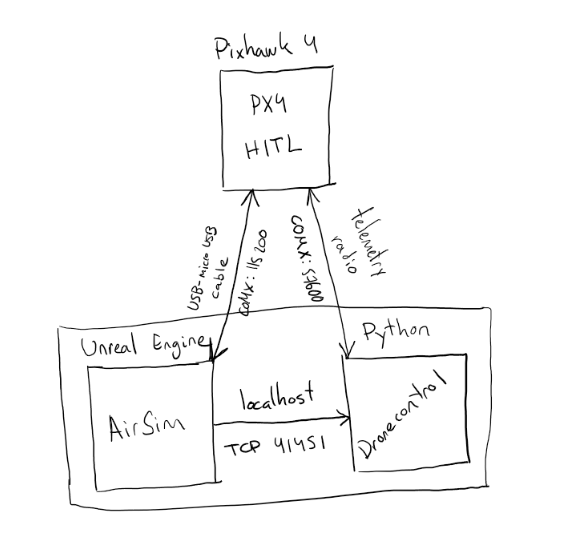
\includegraphics[scale=0.8,keepaspectratio]{img/hitl-connections.png}
  \caption{Connection diagram of how the three systems that interact with each other during HITL simulation.}\label{fig:hitl-connections}
\end{figure}
Figure~\ref{fig:hitl-connections} shows the chosen connections to execute tests in HITL mode.
The Windows machine runs both AirSim and the Python interpreter, which communicate through the localhost network using \gls{TCP}.
The board running PX4 connects to the simulator through a USB to microUSB cable, which is setup to work with a baudrate of 115200, and to the developed program through a telemetry radio running at a baudrate of 57600, both attached to USB ports on the Windows computer accessible through their COM address.

\section{Software architecture}

\begin{figure}
  \centering
  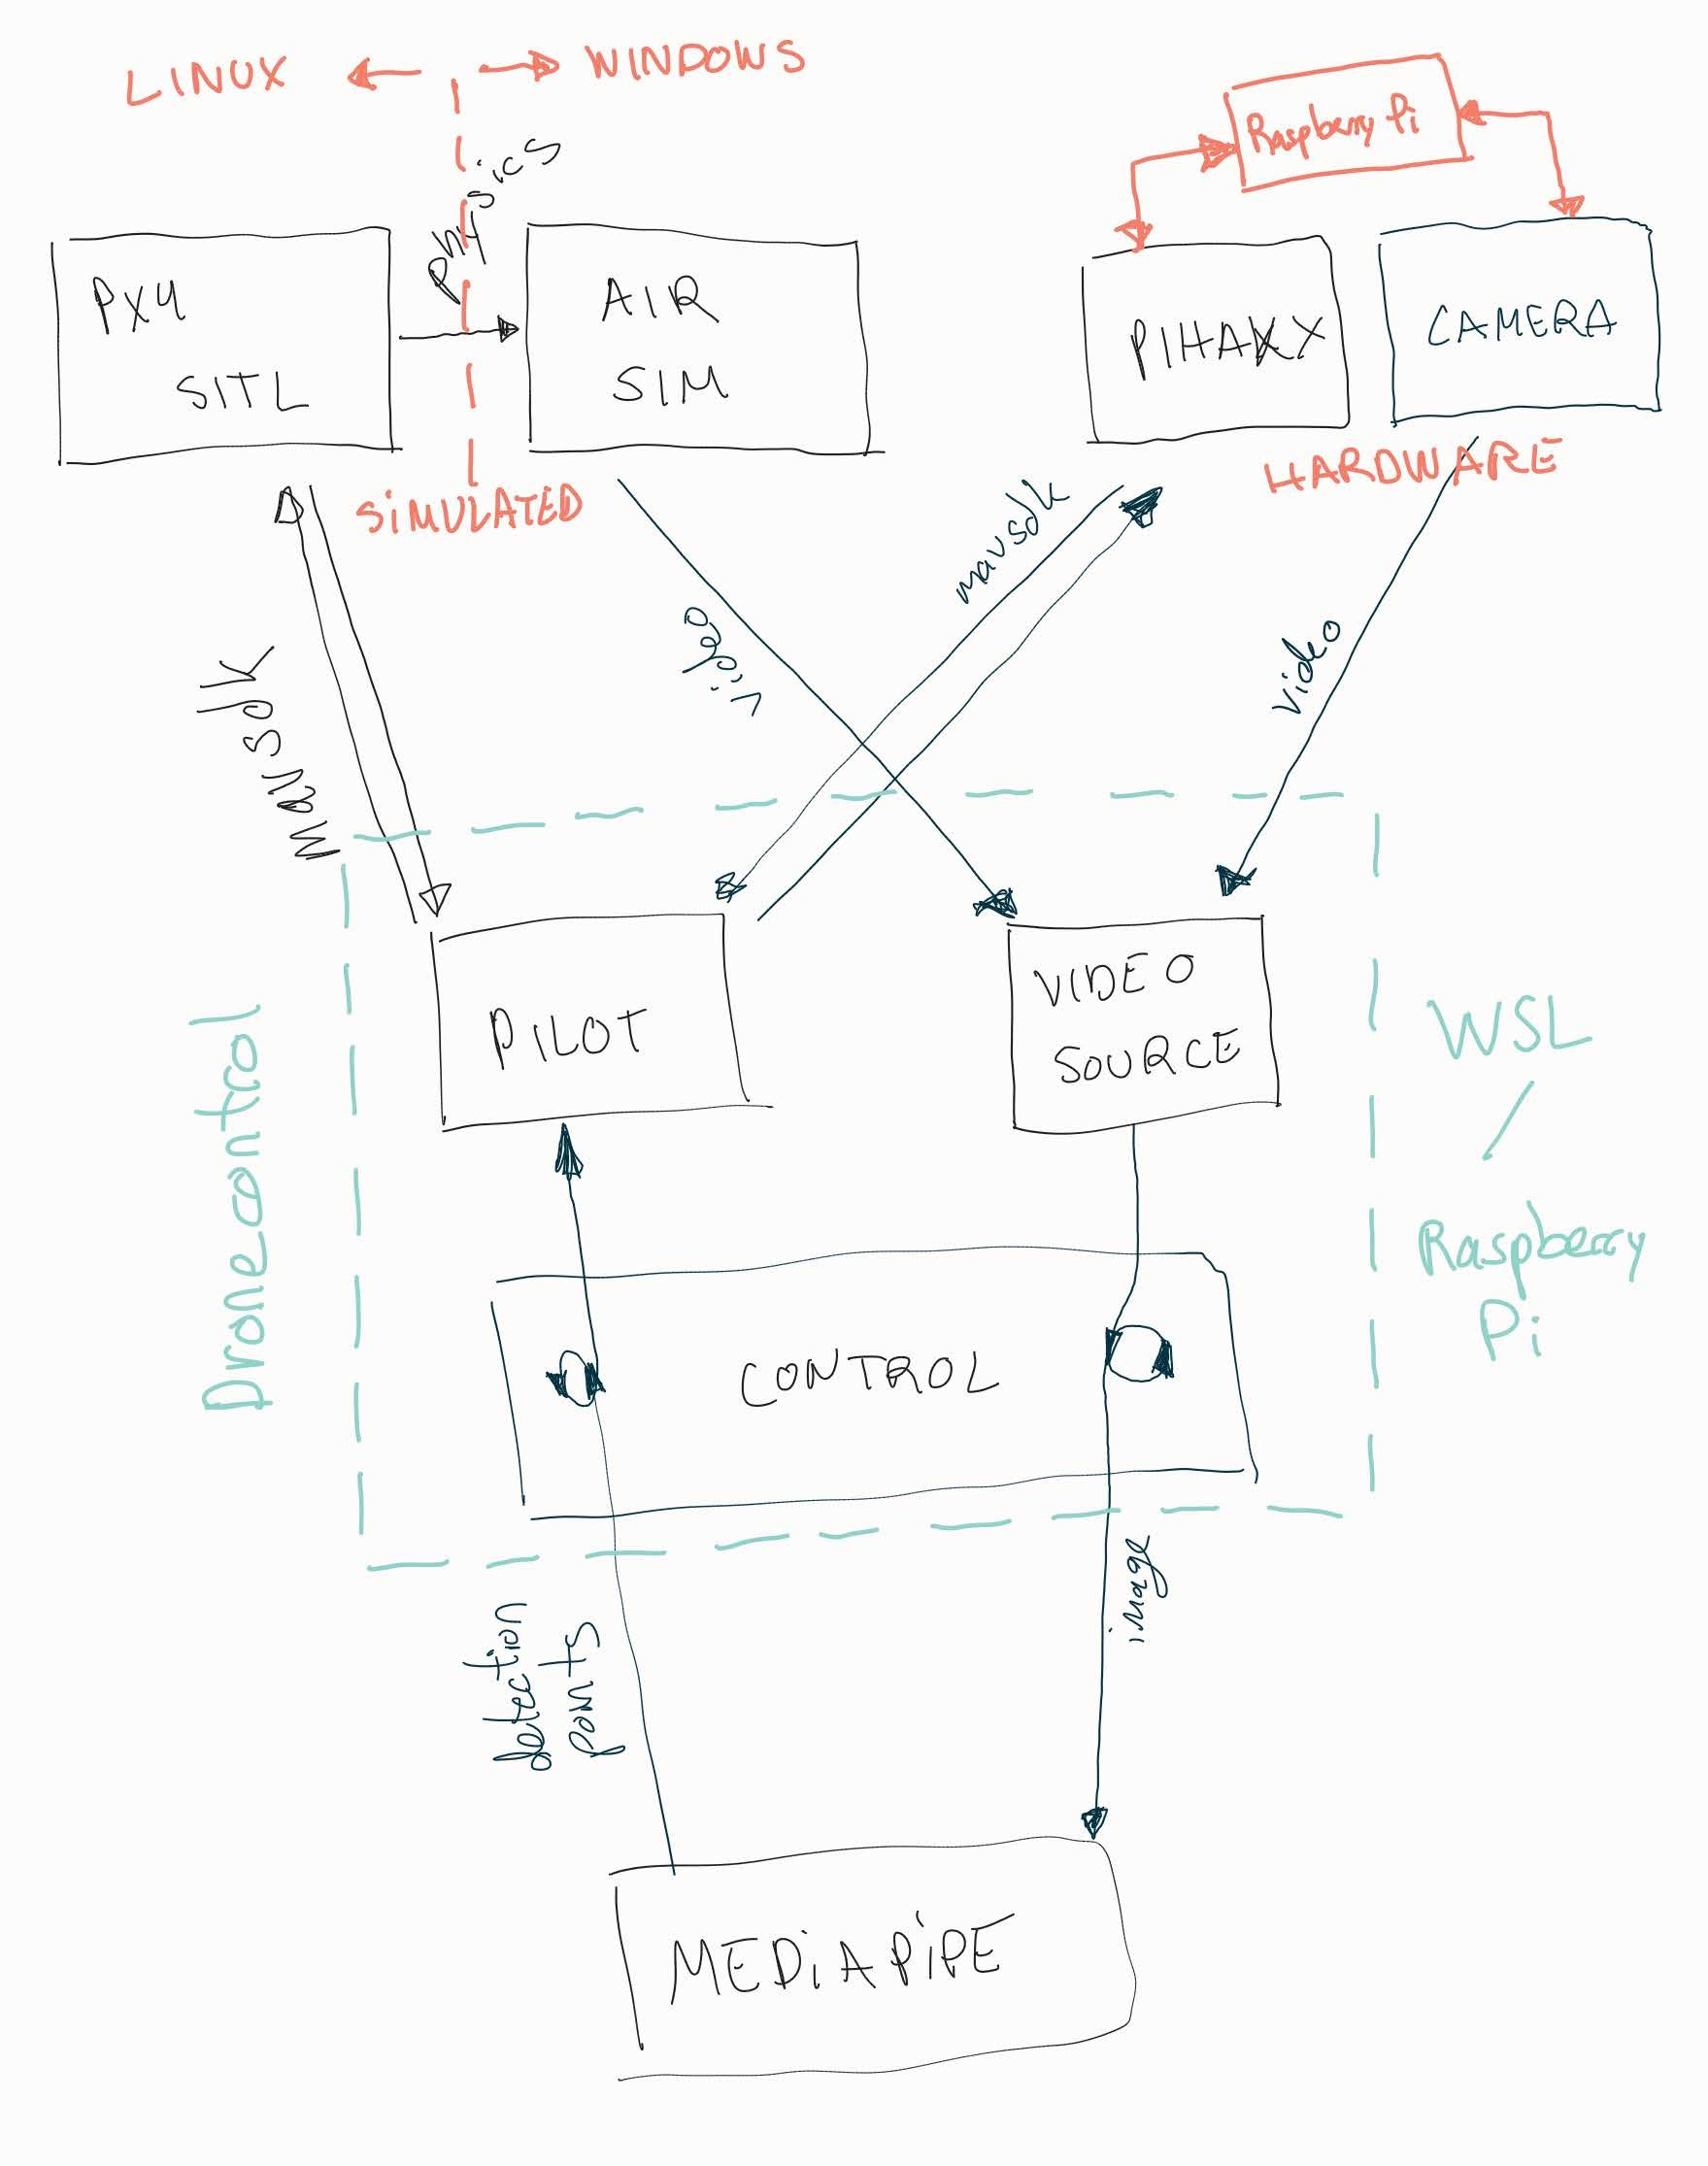
\includegraphics[width=12cm, keepaspectratio]{img/code_diagram.jpg}
  \caption{Structure of the program}\label{fig:architecture}
  \todo[inline]{Draft (use miro for final??)}
\end{figure}

Figure~\ref{fig:architecture} shows the main modules the designed the software is composed of and how it interacts with the external libraries.
The application consists of three basic parts: 
the pilot module, in charge of sending instructions to the flight controller and receiving back information on position and state through the \verb|mavsdk| library, 
a video source module that handles the retrieval of images from different sources and the necessary processing for image analysis, 
and a control module that directs the interaction between the other two to transform the pixel information first into position points through the \verb|mediapipe| library and then into instructions for the pilot.
The upper part of the diagram in Figure~\ref{fig:architecture} shows how the program modules receive input and send instructions to the hardware systems whether these are simulated or not.
Other smaller utilities have also been developed to help test how the systems interact with each other and calibrate different parts of the control behaviour.
\todo[inline]{Command-line interface summary here and link to appendix with full help extract.}
These different parts that make up the dronecontrol app are detailed in the next sections.

\subsection{Pilot module}
The purpose of the pilot module is to provide access to the rest of the application to send and receive messages from the PX4 controller through the MavSDK library.
This library provides a simple asynchronous API for managing one or more vehicles, providing programmatic access to vehicle information and telemetry, and control over missions, movement and other operations.
MavSDK utilizes the python standard library \emph{asyncio} to be able to run coroutines in parallel while waiting for the messages provided through the \emph{MAVLink} communication.
Therefore all calls to the library have to be written as async functions that await the result of one or more polls to the flight stack.

\verb|asyncio| provides support for writing concurrent code using the \verb|async/await| syntax.
It is used as a foundation for multiple Python asynchronous frameworks that provide high-performance network and web-servers, database connection libraries, distributed task queues, etc; 
and provides a set of high-level APIs to run Python coroutines concurrently and have full control over their execution.
The pilot module integrates \verb|mavsdk| and \verb|asyncio| and provides a queue for the control module to send actions to be executed in the vehicle one after another.

Listing~\ref{lst:pilot.connect} shows how to establish a connection to a PX4 vehicle through its physical (serial) or virtual (UDP) address and poll for internal information from the flight controller to decide when the system is ready to receive instructions.
The mavsdk library exposes telemetry and other state information through asynchronous generators, which are defined in python as a convenient way to make asynchronous data producers and accessed with the \mintinline{python}{async for} syntax.


\begin{listing}[h!]
    \caption{Example of how the communication to the flight stack is established through asyncio and the mavsdk library}{}
    \label{lst:pilot.connect}
    \begin{minted}[breaklines, fontsize=\footnotesize, baselinestretch=1]{python}
async def connect(self):
    """Connect to mavsdk server.
       Raises a TimeoutError if it is not possible to establish connection.
    """
    
    if self.serial:
        address = f"serial://{self.serial}"
    else:
        address = f"udp://{self.ip if self.ip else ''}:{self.port}"
    self.log.info("Waiting for drone to connect on address " + address)
    await asyncio.wait_for(self.mav.connect(system_address=address), timeout=self.TIMEOUT)

    async for state in self.mav.core.connection_state():
        if state.is_connected:
            break

    # Wait for drone to have a global position estimate
    async for health in self.mav.telemetry.health():
        if health.is_global_position_ok:
            break
        
    self.log.info("System ready")
    self.is_ready = True
    \end{minted}
\end{listing}

Many of basic operations that can be executed in the flight controller are implemented in the pilot module with error handling and safety checks, like takeoff, landing, return home or manipulating the vehicle flying velocity directly by providing speeds in body coordinates.
These actions can be executed directly or added to a queue that runs in on a loop executing them in the order they are added, waiting until the previous action has finished and the vehicle is in the desired state before starting the next.
The loop that runs this queue can be seen in Listing~\ref{lst:pilot.queue}.
There is a maximum time of 10 seconds that each action can use to run
The loop stops when the asynchronous task it runs on is cancelled with \mintinline{python}{task.cancel()}, which raises a \mintinline{python}{CancelledError} exception in the parallel execution.

\begin{listing}[h!]
    \caption{Loop where the action queue runs on the pilot module. Each action is awaited until it finishes or the timeout time runs out.}{}
    \label{lst:pilot.queue}
    \begin{minted}[breaklines, fontsize=\footnotesize, baselinestretch=1]{python}
async def run_queue(self):
    """
    Run the queue loop.
    
    Queued actions will be awaited one at a time
    until they are finished.
    The loop will sleep if the queue is empty.
    """
    try:
        while True:
            if len(self.actions) > 0:
                action = self.actions.pop(0)
                self.log.info("Execute action: %s", action.func.__name__)
                try:
                    await asyncio.wait_for(action.func(self, **action.args), timeout=10)
                except asyncio.exceptions.TimeoutError:
                    self.log.warning(f"Time out waiting for {action.func.__name__}")
            else:
                await asyncio.sleep(self.WAIT_TIME)
    except asyncio.exceptions.CancelledError:
        self.log.warning("System stop")
    \end{minted}
\end{listing}

\subsection{Video source module}

The objective of the video source module is to provide a collection of classes to retrieve images from different sources,
in a way that they can be exchanged for one another without affecting the rest of the application to facilitate testing and be adaptable running in different environments.
There are three classes of video sources implemented: file, simulator and camera, which inherit from the same \mintinline{python}{VideoSource} base class as shown in Figure~\ref{fig:video-source-inheritance}.

\begin{figure}
  \centering
  
\includegraphics[width=8cm, keepaspectratio]{img/placeholder.png}
  \caption{Diagram of inheritance on the video source classes available to retrieve image data.}\label{fig:video-source-inheritance}
  \todo[inline]{Make inheritance schema}
\end{figure}

The \mintinline{python}{FileSource} class is able to open a video file stored in the companion computer and provides images taken frame by frame from it until the video ends.
This allows the program to replay the image detection algorithms on videos previously captured by the camera tool exposed in section~\ref{subsec:test-tools}.
The \mintinline{python}{CameraSource} class can access a physical camera attached to the computer running the application via USB and provide the frames captured in real time.
Both the file and camera sources employ OpenCV's video capture utilities to take care of the file handling and the camera driver management capabilities respectively.

The simulator source uses AirSim's Python library to communicate with the simulator and retrieve images from a simulated camera attached to the 3D model of the vehicle in Unreal Engine.
It connects automatically through localhost, but it can also be provided with an IP to establish connection to the simulator running on a different computer on the local network, for example when the program runs inside WSL and the simulator runs on its host computer.

\subsection{Control module}
The control module contains the main logic of the application and is in charge of converting the raw images obtained from the video source into commands for the pilot module.
Two different types of control have been implemented.
The first one is a proof-of-concept control solution, described in Section~\ref{subsec:hands}, that runs in offboard mode (see Section~\ref{subsec:offboard}) and translates some predefined hand gestures into simple commands for the aerial vehicle, of which the main purpose is to be able to test the interaction between all the components of the system in a more easily controlled environment, since it uses the simpler configuration of situating the computer with the controller outside of the vehicle.
The second control system consists of a follow solution more applicable to real-life scenarios where the control and the camera is onboard the vehicle and the presence of a person is detected in the images obtained from the perspective of the drone in order to be able to give the flight controller velocity commands to follow said person and maintain it centered in its view.

The process followed in both solutions consists roughly of the same two parts.
First the image is sent to the computer vision and machine learning third-party library that extracts the required features from the image in the form of 2D coordinates.
Afterwards a series of calculations depending on the particular solution are applied to these coordinates to decide which commands are sent to the pilot module.
The third-party library used for computer vision in the program is the mediapipe library described in Section~\ref{subsec:mediapipe}, which offers cross-platform, customizable ML solutions for live and streaming media, specifically its hand and pose detection solutions.

To engage the module in direct control of the vehicle's velocity it is necessary to use a special flight mode defined by PX4 for this purpose, called Offboard Mode \footnote{\url{https://docs.px4.io/main/en/flight_modes/offboard.html#offboard-mode}} (not to be confused with the offboard configuration described in section~\ref{subsec:offboard}).
Offboard mode is primarily used for controlling vehicle movement and attitude, and supports only a very limited set of MAVLink messages. This mode requires position or pose/attitude information to be available to the flight controller, e.g. GPS.
In it, the vehicle obeys a position, velocity or attitude setpoint provided over MAVLink by a MAVLink API (i.e. MAVSDK) running on a companion computer and usually connected via serial cable or wifi.
A stream of setpoint commands must be received by the vehicle at a rate higher than 2Hz prior to engaging the mode and in order to remain in it.
If the message rate falls below 2Hz or the connection is lost the vehicle will stop and, after a timeout, the vehicle will attempt to land or perform some other failsafe action according to the parameters configured.
In order to hold position while in this mode, the vehicle must receive a stream of setpoints for the current position.

The next two sections offer a more complete explanation of the control module used by the two different solutions developed.



\subsection{Proof of concept: hand-gesture solution}
\label{subsec:hands}
The main purpose of this solution is to test that the flow of the application works as expected, both in simulation and in real flight, and that all the systems are capable of establishing the required connections with each other.
For that reason it is designed to be able to be run in real flight with the minimal setup of a built drone with its default components and any computer with a webcam.

\begin{figure}
  \centering
  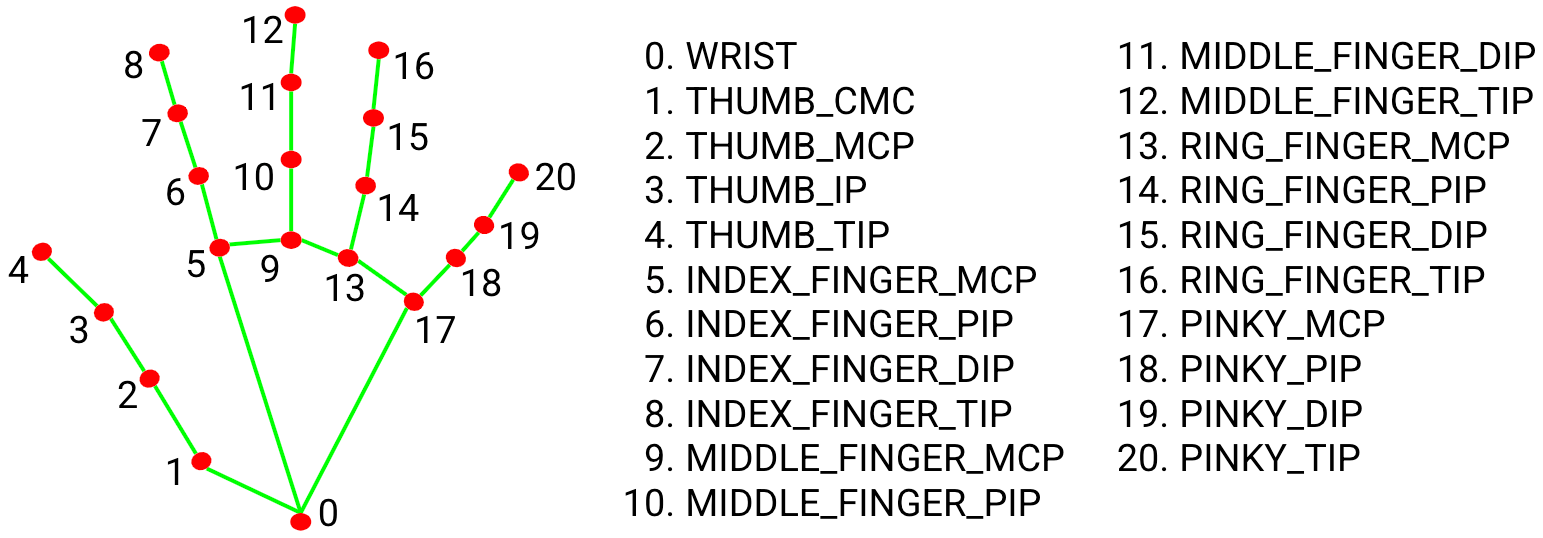
\includegraphics[width=\textwidth, keepaspectratio]{img/hand_landmarks.png}
  \caption{Landmarks extracted from detected hands by the MediaPipe hand solution}\label{fig:hand-landmarks}
\end{figure}

This control module runs on a loop that continuously polls for a new frame from the chosen video source and feeds it to the hand detection functionality from MediaPipe.
If a hand is detected in the images, 2D coordinates are extracted according to the map shown in Figure~\ref{fig:hand-landmarks}.
These landmarks are then converted into different discrete gestures like open palm, closed fist or an specific finger pointing different directions.
When a new gesture is detected, the command assigned to it is queued to the pilot module and executed as soon as the previous commands end their execution.

The conversion between landmarks and gestures is performed by drawing vectors from the base of each of the fingers to their tips as well as from the base of the hand (wrist feature) to the base of the fingers and using the dot product vector operation to calculate the relative angles between each finger and the base of the hand, as shown in Figure~\ref{fig:vector-calcs}.
By comparing the calculated angles to a threshold, it is possible to detect whether each individual finger is extended or folded, as well as the general direction it is pointing towards.
The open hand gesture, for example, can then be defined as all five fingers extended, that is, all five vectors defined by the fingers sharing the same approximate angle with the vector from the base of the hand to that finger.

\begin{figure}
  \centering
  
\includegraphics[width=8cm, keepaspectratio]{img/placeholder.png}
  \caption{Vector calculations}\label{fig:vector-calcs}
\end{figure}

The full list of gestures detected by the program by calculating these angles is as follows:
\begin{itemize}
    \item No hand: happens when no landmarks are able to be extracted from the image. As a safety feature, in this case the vehicle stops whichever previous commands it had in its queue and goes into hold flight mode, where it just hovers in the air maintaining its position.
    \item Open hand: it is detected when all five fingers are extended, as if gesturing stop, and makes the drone land at its current position.
    \item Fist: it is detected when all five fingers are folded and makes the drone arm and takeoff. If the drone is already in the air nothing happens.
    \item Index finger pointing up: it is detected when only the index finger is extended and it is pointing roughly towards the top of the image ($\pm 30$ degrees) and makes the drone go into offboard mode, where it is possible to receive direct velocity commands.
    \item Index finger pointing to the right: same as above but pointing to the right of the image and makes the drone roll towards its right side at a speed of 1 m/s.
    \item Index finger pointing to the left: same as above but the drone rolls towards its left side.
    \item Thumb pointing to the right: it is detected when index finger is extended up (to maintain the drone in offboard control) and the thumb is extended pointing towards the right of the screen. This gesture makes the drone pitch forward at a steady speed of 1 m/s.
    \item Thumb pointing to the left: same as the previous gesture, but the drone pitches backward when the thumb point to the left of the screen.
\end{itemize}

\todo[inline]{Include some code for the module after cleanup, vector calcs and/or running loop}
\todo[inline]{Include diagram of angles for each pointy gesture ?????}
\todo[inline]{Include images of program output image with drawn lines for gestures}


\subsection{Final solution: human following}
\label{subsec:follow}

\subsection{Other utilities}
\label{subsec:test-tools}


\cleardoublepage